\documentclass{article}
\usepackage[english]{babel}
\usepackage[utf8]{inputenc}

\usepackage{mlmodern}
\usepackage[T1]{fontenc}
\usepackage{graphicx}
\usepackage{subfigure}
\usepackage{float}
\usepackage{amsmath, amsfonts, amssymb, amsthm}
\usepackage{hyperref}
\usepackage{dirtytalk}
\usepackage{biblatex}

\addbibresource{refs.bib}

\newtheorem{defi}{Definition}
\newtheorem{theorem}{Theorem}

\newcommand{\N}{\mathbb{N}}
\newcommand{\R}{\mathbb{R}}
\newcommand{\C}{\mathbb{C}}
\newcommand{\e}{\mathrm{e}}

\title{Construction of epicycloids from sequences on the unit circle}

\author{Felix Widmaier}

\date{}

\begin{document}

\maketitle

\begin{abstract} 
\noindent
The main result of this essay is probably already well known. The essay is mainly for entertainment and should serve as an essay 
for scientific scepticism in mathematics. We generalise a theorem of L. Cremona, according to which the cardioid is the envelope of 
a pencil of lines \cite{cremona}. The lines are constructed as follows: If $n\in\mathbb{N}$ then we number $2n$ points on the 
unit circle consecutively. These points must also divide the circle into $2n$ equal parts. Then we draw the chords 
$(1,2), (2,4),\ldots,$. The envelope of these chords is then the cardioid, which we will call the 1-epicycloid in the following. 
Let $k\in\N$. In this essay we will proof that the envelope of the pencil of $kn$ lines given by chords of the form 
$(a_i, a_{i+1})$ where $a_{i+1} = k\cdot a_i$  and $a_1 =1$ for some $k\in\mathbb{N}$ is the $(k-1)$-epicycloid.
\end{abstract}

\noindent\paragraph{Keywords}{geometry; epicycloids; \textit{recreational mathematics}; \textit{scientific scepticism}}\\


\section{Motivation and main result}
There are not many esoteric hypotheses or conspiracy narratives that concern mathematics or at the very least attempt to explain the \say{magic} 
with mathematics. These often involve numerology, which has fascinated people for millennia, or at least those with an esoteric inclination. 
Criticism of numerology is at least as old as numerology itself. This essay is intended to present an exemplary essay of scientific scepticism 
on the basis of \say{vortex math}. As the author, I am primarily concerned with the entertainment aspect offered by the mathematical questions 
of the main result and with calling out bullshit. At first, this may seem like reaching for low-hanging fruit, since such esoteric narratives do 
not have much to offer academically and intellectually, to put it euphemistically. However, for the sake of elucidation alone, such narratives 
should be reported and this nonsense put to a stop. But first, let's take a quick look at \say{vortex math}. For this I mainly used the 
source \cite{omnia}, since other sources mostly \say{argue} analogously. Other sources are for example \cite{powell,steinhauser}.\newline

Nikola Tesla is often quoted by people with esoteric inclinations as saying \say{If you only knew the magnificence of the 3, 6 and 9, then 
you would have the key to the universe} \cite{omnia,goodreads}. This quotation is usually justified afterwards by the fact that the digital 
root\footnote{Where the digital root of a number is the iterative summation of the digits until you arrive at a one-digit number. In doing so, 
one can easily consider the following. Let $l\in\N$ and $d\in\N$ be the digital root of $l$. Then $d$ is the remainder which results from the integer 
division of $l$ by $9$} of $2^n$ for $n\in\N$ never equals $3$, $6$ or $9$.\footnote{No further, deeper justification is provided. It is only loose 
associations and empty assertions.} Before you know it, you are already in the midst of what esotericists call \say{vortex math}. 
The basis of \say{vortex math} is the sequence $1, 2, 4, 8, 5, 1, 2,\ldots$ In other words, the sequence of the digital roots of $2^n$. If the numbers 
from $1$ to $9$ are plotted on a circle as on a clock with 9 at the top, and then secants of two consecutive numbers in the sequence of digital roots 
of $2^n$ are drawn, a symmetrical figure is obtained within the circle, see figure \ref{fig:vvortex}. The resulting plot is referred to as 
\say{the symbol of enlightenment} by Marko Rodin, to whom the original idea of \say{vortex math} traces its origins \cite{omnia, powell}.
\begin{figure}[ht]
    \centering
    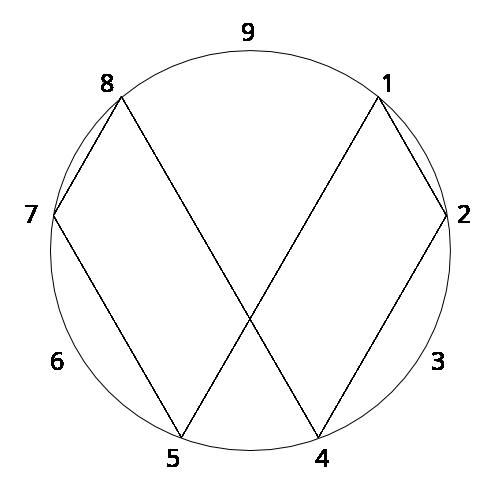
\includegraphics[scale=0.25]{images/vortex.png}
    \caption{``The symbol of enlightenment''}
    \label{fig:vvortex}
\end{figure}
Since this figure, with a little imagination, is reminiscent of the symbol for infinity, esotericists interpret all kinds of things into this construction. 
Some even conclude that the sequence of digital roots of $2^n$ thus describes creation itself.\newline

These are, of course, blatant leaps of thought, which unfortunately could not really be substantiated in any source I could find. However, one finds a certain 
magical thinking that is typical of esotericism \cite{Lamberty_Nocun_2022}. In addition, we find here a philosophy of mathematics that can be summarised 
like this: Numbers render the environment and vice versa. Unlike as it is typical for empiricism that numbers come from measurements. Numbers as they are can 
therefore influence physical reality - this is magical thinking. Whereby the magic spells have been exchanged for numbers. However, this view is typical of 
esotericism and numerology. Moreover, this \say{model} is also mathematically very limited. As a mathematician, one quickly gets the idea of simply choosing 
a base other than $10$ and then considering the digital roots of $2^n$ in each case. The resulting construction can be seen in 
figure \ref{fig:cremona}.\footnote{When choosing the base to be $62$ for example.} Another question that can be asked is why we have so far only considered 
the digital roots of $2^n$. We could just as well generalise and consider digital roots of $k^n$, where $l\in\N$. If you play with the numbers, you quickly 
notice the following astonishing result: the envelope of each of the drawn lines is an epicycloid. The main result, which is formulated in the next 
subsection, precisely shows this observation.
\subsection{Main result}
We are finally leaving the intellectually dull field of esotericism. Now we will devote ourselves to some more serious mathematics and ask real mathematical questions.
\begin{defi}
    Let $k\in\N$. We call the curve generated by
    \begin{equation}\label{eq:epi}
        \psi\colon[0,2\pi]\to\C,\ \varphi\mapsto\e^{i\varphi}\left(1+\frac{1}{k}+\frac{1}{k}\cdot\e^{ik\varphi}\right)
    \end{equation}
    the $k$-epicycloid.
\end{defi}
The $k$-epicycloid is obtained by tracing the path of a fixed point on a circle with radius $\frac{1}{k}$ which rolls around the unit circle. 
Figure \ref{fig:epicycloids} gives some example plots of $k$-epicycloids.
\begin{figure}[h]
    \centering
    \subfigure[$k=1$]{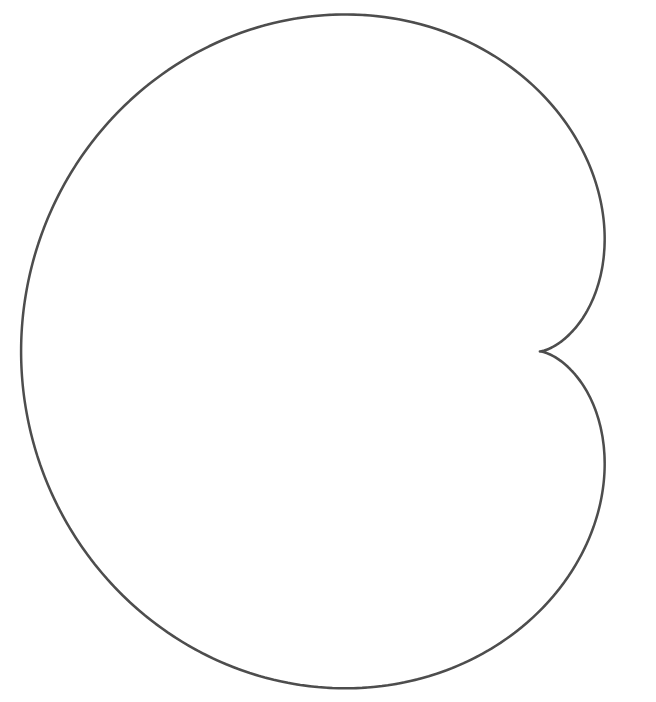
\includegraphics[width=0.15\textwidth]{images/epi1.png}}\hspace{1.2cm}
    \subfigure[$k=2$]{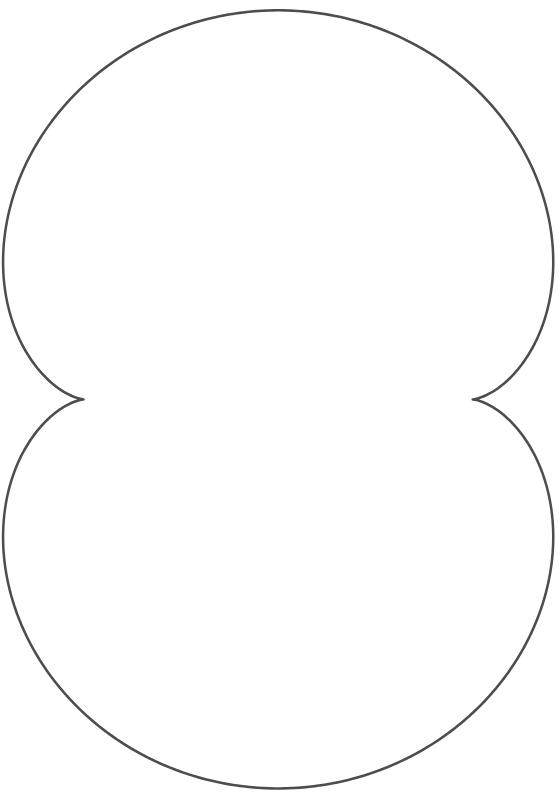
\includegraphics[width=0.12\textwidth]{images/epi2.png}}\hspace{1.2cm}
    \subfigure[$k=3$]{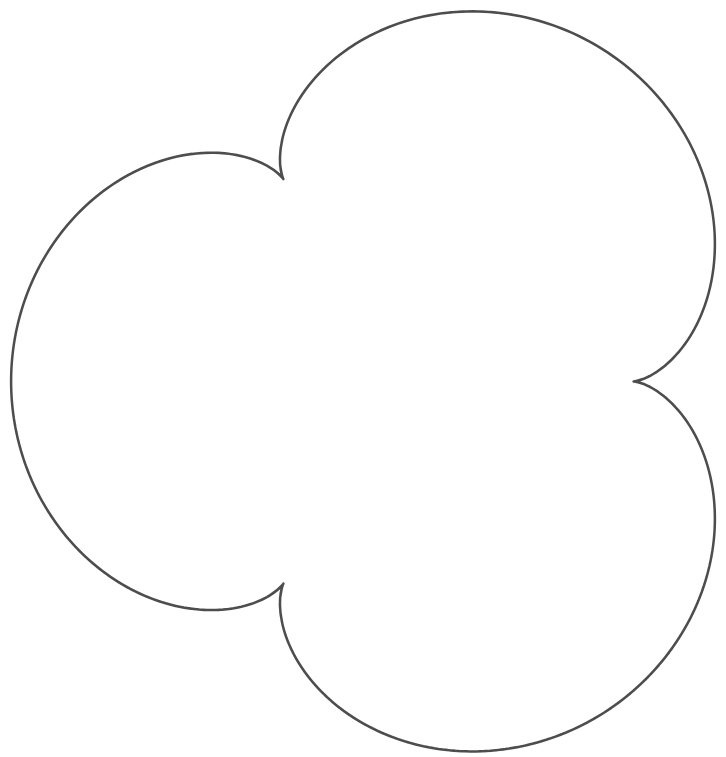
\includegraphics[width=0.155\textwidth]{images/epi3.png}}\hspace{1.2cm}
    \subfigure[$k=4$]{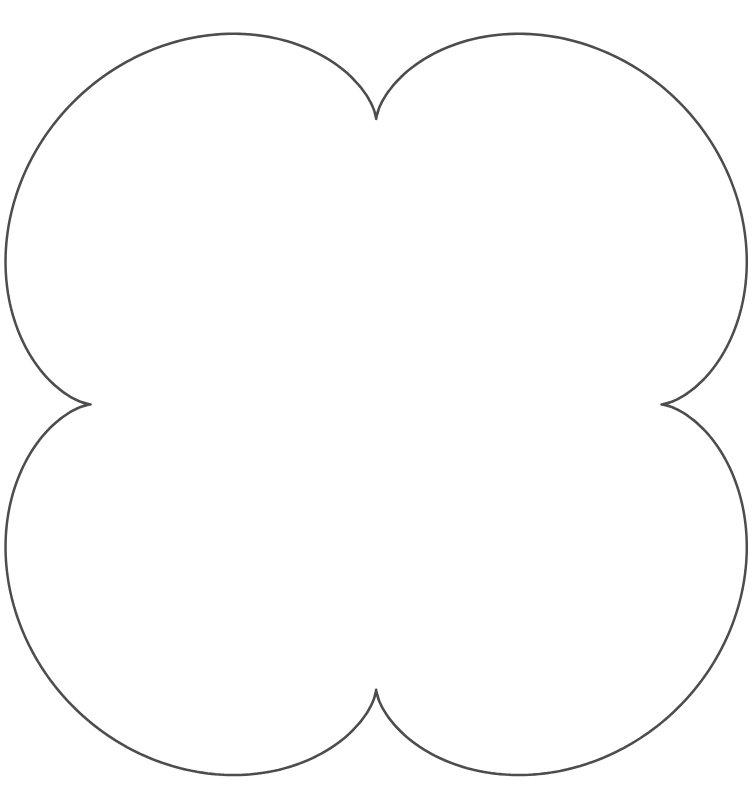
\includegraphics[width=0.15\textwidth]{images/epi4.png}}
    \caption{Plots of $k$-epicycloids  with ascending $k$}
    \label{fig:epicycloids}
\end{figure}\newline\noindent
In this essay we will give a proof of the following theorem
\begin{theorem}\label{thrm:epi}
    Let $n,k\in\N$. Let $\{z_i\}_{i=1}^{kn}$ be points on the unit circle which divide the unit circle into $kn$ sections and are numbered 
    consecutively. We denote the chord through $z_a$ and $z_b$ with $(a,b)$ where $1\leq a,b\leq kn$ and $a\neq b$. Then the envelope of the 
    pencil of chords $\{(a_i, a_{i+1})\mid a_1 = 1, a_{i+1}=k\cdot a_i, 1\leq i\leq kn\}$ is the $(k-1)$-epicycloid.
\end{theorem}
\newpage
This is a generalisation of the result of L. Cremona, as the result from L. Cremona is essentially a special case of Theorem \ref{thrm:epi} where $k=2$. 
Whereby the envelope is the $1$-epicycloid. This can be visualised quite nicely. If we plot an arbitrary number of points on the unit circle and draw 
the chords as described above, considering only the remainder when dividing by the number of points, we get very visually stunning pictures 
(see figure \ref{fig:cremona}).
\begin{figure}[ht]
    \centering
    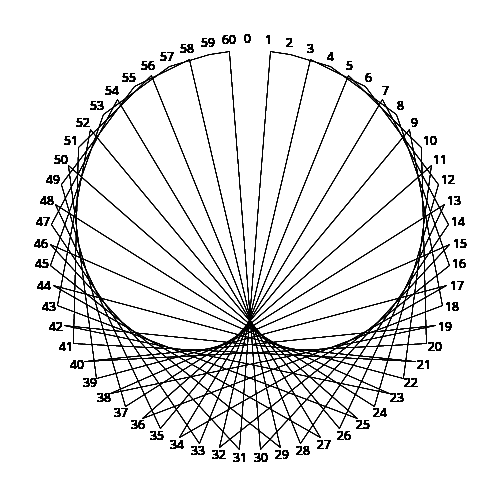
\includegraphics[scale=0.3]{images/param2mod61.png}
    \caption{The pencil of lines with $n=61$, $k=2$ and $a_{i+1} = k\cdot a_i\mod 61$ and $a_1=1$}
    \label{fig:cremona}
\end{figure}

We can proceed in the same fashion for larger numbers, see figure \ref{fig:thrm}. One can easily see the $(k-1)$-epicycloids emerging from the patterns of lines:
\begin{figure}[h]
    \centering
    \subfigure[$k=3$]{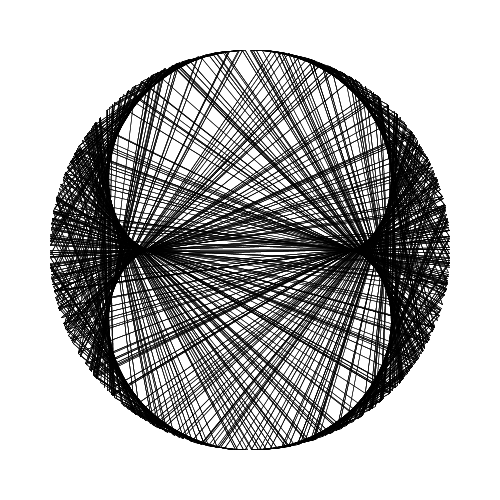
\includegraphics[width=0.3\textwidth]{images/param3mod5123.png}}
    \subfigure[$k=4$]{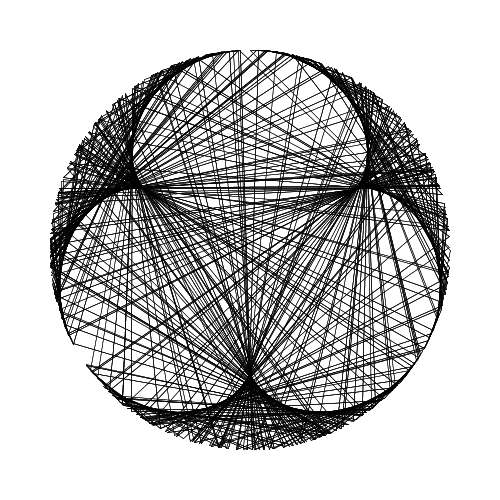
\includegraphics[width=0.3\textwidth]{images/param4mod5123.png}}
    \subfigure[$k=5$]{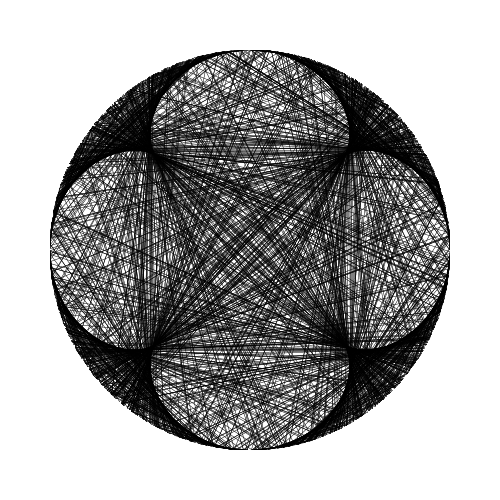
\includegraphics[width=0.3\textwidth]{images/param5mod5123.png}}
    \caption{Plots generated with $n=5123$}
    \label{fig:thrm}
\end{figure}
\newpage
\section{Proof of the theorem}
\begin{proof}[Proof of Theorem \ref{thrm:epi}] Let $k\in\N$ and $\varphi\in\R$ such that 
	$\varphi\neq \frac{2\pi n}{k}$ for all $n\in\N$. From \eqref{eq:epi} we find the tangent to the $k$-epicycloid in the 
	point $\psi(\varphi)$. The tangent is given by
    \begin{align}\label{eq:tangent}
        T_{\varphi}\colon\R\ni t\mapsto i\left(\dfrac{1}{k}+1\right)\left(\e^{i\varphi}+\e^{i\varphi(k+1)}\right)\cdot t+\psi(\varphi)\in\C.
    \end{align}
    We can also find the parametrization of the chord that passes through 
    $\left(1 + \dfrac{2}{k}\right)\e^{i\varphi}$ and $\left(1 + \dfrac{2}{k}\right)\e^{i\varphi(k+1)}$. This chord is given by
    \begin{align}\label{eq:chord}
        S_{\varphi}\colon\R\ni t\mapsto \left(1+\dfrac{2}{k}\right)\left(\e^{i\varphi(k+1)}-\e^{i\varphi}\right)\cdot t + \left(1+\dfrac{2}{k}\right)\e^{i\varphi}\in\C.
    \end{align}
    It is now sufficient to show that the lines parametrized through \eqref{eq:tangent} and \eqref{eq:chord} are the same. By
    \begin{align*}
        i\frac{\e^{i\varphi}+\e^{i\varphi(k+1)}}{\e^{i\varphi(k+1)}-\e^{i\varphi}} = \operatorname{cot}\left(k\frac{\varphi}{2}\right)\in\R
    \end{align*}
    we find that both lines have the same slope. Furthermore we see that 
    \begin{align*}
        \psi(\varphi) = S_{\varphi}(t)
    \end{align*}
    is equivalent to $t = \frac{1}{2+k}$. Thus the lines \eqref{eq:tangent} and \eqref{eq:chord} share at least one point. Thus they are equal and the assertion follows.
\end{proof}
\section{Conclusion}
While I acknowledge that this text is not completely presupposition-free in order to understand it in its entirety, I hope that I have sparked some 
interest in you, the reader, and that you feel entertained by this text. I also hope that after you have seen the main result, you have also seen 
how limited the approach of the esotericists is to choose the base ten and to double the numbers. Mathematics is such a particularly beautiful 
field of study with extremely many wonderful results. It would be a pity if esoteric narratives like this were to pollute this beautiful field of study. 
Bullshit must be called out whenever it is seen. While investigating all this I came upon this \cite{theproblemsite} website which I can recommend for 
further reading into this topic when you are interested in more serious mathematical questions.
\newpage
\printbibliography
\end{document}
